\section{Research Goal and Research Question}

\subsection*{Motivation}

The project is intended to make the same synthetic generator useful both as a
\emph{prior} and as a \emph{benchmark}. Following the terminology used by
DoTime \citep{thumm2026dotime}, the prior is the distribution of synthetic
tasks used to train a model, while the benchmark is a fixed set of generated
tasks used to evaluate it. Because the equation and all sampled components are
known, the generator can provide supervision that is unavailable in real
time-series data.

As a prior, the generator could be used to pretrain a foundation model for
more than future-value prediction. From the same encoded time series, the
model could forecast the horizon, recover the equation that generated the
series through symbolic regression, and predict the expected uncertainty due
to the innovation added at each step. The exact future innovation is random;
the learnable quantity is the error distribution expected before the future is
observed.

The generator will also produce explanation ground truths for training
explanation-aware models. SHAPformer illustrates the general idea at a high
level: during training, random feature coalitions are hidden, so the model
learns to forecast from different subsets of the input. At inference, the
differences between forecasts made with and without each group provide its
SHAP- or Owen-style contribution \citep{hertel2026shapformer}. Its synthetic
ground-truth explanations are used to evaluate the resulting contributions.
The proposed framework will generalize this idea by supplying coalition masks
and explanation targets that can be used either for masked training or as
direct supervision for an explanation head in other architectures.

As a benchmark, the same generator will produce fixed evaluation datasets with
hidden equations and known explanation references. These datasets will make it
possible to evaluate separately whether a model predicts the future, recovers
the generating equation, represents the expected innovation, and identifies
the variables and past time steps responsible for each forecast.

\begin{figure}[H]
\centering
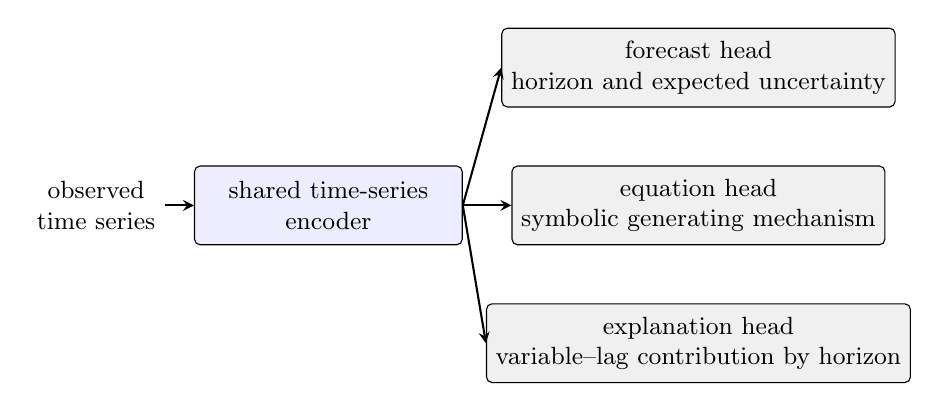
\begin{tikzpicture}[
    block/.style={draw,rounded corners=2pt,fill=blue!7,
        minimum width=3.4cm,minimum height=1.0cm,align=center,font=\small},
    head/.style={draw,rounded corners=2pt,fill=black!6,
        minimum width=4.1cm,minimum height=1.0cm,align=center,font=\small},
    flow/.style={->,>=stealth,draw,line width=0.75pt}
]
    \node[font=\small,align=center] (input) at (-5.2,0)
        {observed\\time series};
    \node[block] (encoder) at (-2.25,0)
        {shared time-series\\encoder};
    \node[head] (forecast) at (2.45,1.75)
        {forecast head\\horizon and expected uncertainty};
    \node[head] (equation) at (2.45,0)
        {equation head\\symbolic generating mechanism};
    \node[head] (explanation) at (2.45,-1.75)
        {explanation head\\variable--lag contribution by horizon};

    \draw[flow] (input)--(encoder);
    \draw[flow] (encoder.east)--(forecast.west);
    \draw[flow] (encoder.east)--(equation.west);
    \draw[flow] (encoder.east)--(explanation.west);
\end{tikzpicture}
\caption{Conceptual multi-task model enabled by the synthetic prior. A shared
encoder feeds a forecasting head, an equation-recovery head, and an
explanation head. The generator supplies the training target for each output,
and the benchmark uses the same information as evaluation ground truth.}
\label{fig:dual-prior-benchmark-motivation}
\end{figure}

\subsection{Research Goal}

The goal of this thesis is to design, implement, and validate a configurable
synthetic benchmark for discrete-time time series. Each dataset will be
produced by a fully known generative mechanism from which several compatible
levels of explanation ground truth can be derived. The benchmark will support
the systematic evaluation of three method families: forecasting models,
symbolic system-identification methods, and XAI techniques. The central
evaluation question is whether these methods recover, use, and explain the
true temporal dependencies of the process.

The generator family will progress from simple to more demanding mechanisms,
including autoregressive dependencies, cross-variable and variable--lag
interactions, nonlinear terms, multiple temporal scales, regime changes,
irrelevant variables, and stochastic components. Depending on the mechanism,
the resulting references will include binary structural dependencies, exact
signed coefficients, realized local coefficient--input contributions, and
attribution-based explanations such as generator-level Shapley values. These
references will be indexed at the target, source-variable, lag, instance, and,
when the generator produces multiple future values, forecast-horizon levels.

Following the expression-first strategy of \citet{dascoli2022deep} and the
learned tree-prior alternative of \citet{meznar2023efficient}, the formula
sampler will construct a valid symbolic tree before generating observations.
The retained tree will act as an executable data-generating function and as the
canonical record from which the benchmark derives its structural,
coefficient-level, local-contribution, and attribution-based references.
Following \citet{bendinelli2023controllable}, an optional retrieval protocol
will expose controlled subsets of this record as hypotheses and measure how
mechanism recovery changes when prior information is complete, partial,
missing, or partially incorrect.

The resulting framework will provide controlled and reproducible comparisons
of predictive accuracy, mechanism recovery, and explanation accuracy. It will
also support tests of whether a black-box forecaster relies on the same
temporal relationships as the true generator or as a symbolic model identified
independently from the generated observations.

\subsection{\texorpdfstring{\hspace{0.45em}Research Question}{Research Question}}

\begin{quote}
\textbf{How can synthetic discrete-time time-series generators with known
generative mechanisms and explanation ground truths be used to benchmark the
ability of forecasting, system-identification, and explainability methods to
recover, use, and explain the underlying temporal dependencies?}
\end{quote}

\paragraph{Three sources of disagreement.}
Let $x$ be a forecasting input, $g$ the known generator, $f$ a forecaster
trained on observations from $g$, and $\widehat g$ a symbolic mechanism
identified independently from those observations. The benchmark separates the
following quantities:

\begin{align}
\varepsilon_{\mathrm{forecast}}(x)
&=d_y\!\left(f(x),g(x)\right),
\label{eq:forecast-error}\\
\varepsilon_{\mathrm{mechanism}}^{*}
&=d_{\mathcal M}\!\left(\mathcal M(\widehat g),\mathcal M(g)\right),
\label{eq:mechanism-error}\\
\varepsilon_{\mathrm{explanation}}(x)
&=d_{\mathcal E}\!\left(A(f,x),E_f(x)\right).
\label{eq:explanation-error}
\end{align}

\noindent\textsuperscript{*}\emph{Applicability of the mechanism error:}
this quantity is evaluated when the method exposes an explicit representation
$\mathcal M(\cdot)$ that can be aligned with the known generator, as occurs in
symbolic system-identification methods and explainable-by-design forecasters.
For an explainable-by-design forecaster, $\mathcal M(\widehat g)$ in
Eq.~\ref{eq:mechanism-error} is replaced by $\mathcal M(f)$. Post-hoc
attribution methods are evaluated through the explanation comparisons in
Eqs.~\ref{eq:explanation-error}--\ref{eq:symbolic-agreement}.

Equation~\ref{eq:forecast-error} measures whether the forecaster returns the
same future values as the generator. Equation~\ref{eq:mechanism-error} measures
whether system identification recovers the generator's structure, lags,
coefficients, nonlinear terms, and regimes at the level represented by
$\mathcal M$. Equation~\ref{eq:explanation-error} measures whether an XAI
method faithfully describes the mechanism actually used by the trained
forecaster; $E_f(x)$ denotes the corresponding model-level reference.

An explainable-by-design forecaster that exposes generator-compatible
source--lag coefficients can also be evaluated through
$d_{\mathcal M}(\mathcal M(f),\mathcal M(g))$, as in the coefficient-recovery
setting studied with DCIts \citep{baric2026dcits}. For a black-box forecaster,
two additional comparisons answer complementary questions:

\begin{align}
\varepsilon_{\mathrm{generator\ agreement}}(x)
&=d_{\mathcal E}\!\left(A(f,x),E_g(x)\right),
\label{eq:generator-agreement}\\
\varepsilon_{\mathrm{symbolic\ agreement}}(x)
&=d_{\mathcal E}\!\left(A(f,x),E_{\widehat g}(x)\right).
\label{eq:symbolic-agreement}
\end{align}

The first comparison tests end-to-end agreement between the black-box
explanation and the true process explanation; it combines any mismatch learned
by $f$ with the behavior of the XAI method. The second tests agreement with an
independently recovered symbolic explanation; its interpretation is paired
with the mechanism-identification error in Eq.~\ref{eq:mechanism-error}. A
small symbolic-agreement error becomes evidence about the true mechanism when
$\widehat g$ also achieves a small mechanism-identification error. Together,
these quantities separate accurate forecasting, recovery of the generating
rule, and faithful explanation of the predictor while allowing their
relationships to be studied explicitly.

\subsection{Benchmark Requirements}
\label{sec:benchmark-requirements}

The benchmark requirements distinguish three kinds of commitment. A
\emph{core requirement} defines behavior that the first complete library must
provide; a \emph{research requirement} identifies a methodological decision
that must be resolved and documented during development; and an
\emph{extension point} keeps the implementation open to later additions
without expanding the experimental scope of this thesis. This distinction is
important because the principal contribution is the generation of executable
time-series mechanisms and their explanation ground truths. General-purpose
grammar design and unrestricted user-defined operators remain extension
points.

\subsubsection{Fixed grammar and reproducible mechanism sampling}

\paragraph{R1: fixed and versioned grammar.}
The project will define one fixed initial vocabulary of constants, lagged
variables, unary operators, binary operators, and mechanism-level constructs.
Users will configure how mechanisms are sampled from this vocabulary, while
the vocabulary itself remains controlled by the project. Every generated
dataset will record a grammar version. Internally, operators will be
registered through a modular interface so that later versions can extend the
grammar without changing the public contract of the first benchmark.

\paragraph{R2: deterministic random generation.}
A global seed, complete generation configuration, library version, and
execution backend will determine the generated mechanisms, coefficients,
initial conditions, innovations, trajectories, windows, and stochastic
explanation estimates. Each artifact will receive a named random stream
derived from stable identifiers such as the mechanism, trajectory, window,
and explanation method. Consequently, changing the number of data-loading
workers or their completion order will preserve the identity and contents of
every indexed example. Repeated execution on the same backend will target
bitwise equality; comparisons across numerical backends will use a declared
floating-point tolerance.

\paragraph{R3: separation between mechanisms and trajectories.}
A mechanism record will contain the expression tree, lag assignments,
coefficients, noise law, and any regime-transition rule. One mechanism may
generate several trajectories. These trajectories share the same symbolic
tree and sampled mechanism parameters while using independently seeded initial
conditions and innovation realizations. This hierarchy supports the study of
whether a method recovers a persistent generating rule rather than properties
of one particular realization:
\[
\boxed{
\text{mechanism}
\longrightarrow
\{\text{trajectory}_{1},\ldots,\text{trajectory}_{K}\}
\longrightarrow
\{\text{forecasting windows}\}.
}
\]
Each window will retain identifiers linking it to its trajectory and canonical
mechanism.

\subsubsection{Controlled and randomly covered difficulty}

\paragraph{R4: two complementary descriptions of difficulty.}
The benchmark will store both \emph{designed difficulty}, determined by the
sampled mechanism, and \emph{measured difficulty}, determined from the
realized forecasting task. Designed difficulty includes tree depth, operator
count, interaction order, number of active variables, lag distance, temporal
scales, recursion depth, regime changes, and the configured noise level.
Measured difficulty includes forecastability statistics, oracle uncertainty,
and the excess error of a fixed panel of reference forecasters over the known
generator.

This separation avoids treating all hard examples as equivalent. A
white-noise process has a simple structural rule but high irreducible
uncertainty, whereas a noiseless nonlinear recurrence can be structurally
complex while remaining deterministic. Difficulty is therefore recorded for
a specified input length, observed-variable set, loss, and horizon. The same
trajectory can be easy at $h=1$ and difficult at a longer horizon.

Related work supplies useful but complementary precedents. SynTSBench controls
temporal pattern families, irregularities, dependencies, and theoretical
optima in order to diagnose forecasting capabilities
\citep{tan2025syntsbench}. The difficulty-conditioned generator of
\citet{cazaux2026synthetic} uses a scalar to alter component balance,
harmonics, regime changes, and noise, and samples named easy, medium, hard, and
uniform distributions. Its downstream ablation also shows that generator
difficulty labels alone need not create proportionally separated forecasting
errors. Data-driven forecastability can additionally be characterized through
spectral predictability and Lyapunov stability \citep{wang2025forecastability}
or through the task-aligned spectral-coherence score of
\citet{feng2025predictability}. These results motivate calibration rather than
assigning difficulty from expression size alone.

\paragraph{R5: random generation with calibrated coverage.}
The default benchmark suite will first sample a target difficulty stratum and
then sample mechanisms from its internal prior. A calibration stage will
measure the realized examples, adjust or relabel them, and freeze versioned
thresholds. The released suite will report the intended stratum and the
measured difficulty descriptors, permitting both a balanced easy--medium--hard
comparison and analysis along the individual axes. Establishing the precise
calibration score and thresholds is a research requirement of the thesis.

\subsubsection{Horizon-aware explanation ground truths}

\paragraph{R6: a separate reference for every forecast step.}
Every explanation ground truth will retain the forecast-horizon axis. For a
source variable $j$, historical offset $d$, and forecast step $h$, the
reference answers whether and how $x_{j,\tau-d}$ affects $g_h(x)$. The canonical
tensor organization is therefore
\[
\boxed{
\text{example}\times
\text{target}\times
\text{horizon}\times
\text{source variable}\times
\text{historical offset},
}
\]
with additional value or method dimensions only when required by a specific
ground-truth family. Aggregation over $h$ will be a reported summary rather
than a replacement for the horizon-resolved reference.

\paragraph{R7: propagation through recursive rollouts.}
When a later forecast uses an earlier generated value, its explanation will be
propagated back to the original observed window. For example, if $g_2(x)$ uses
$g_1(x)$, its input gradient includes both a direct path and the path through
the first forecast:
\begin{equation}
\frac{\partial g_2(x)}{\partial x_{j,\tau-d}}
=
\left.
\frac{\partial g_2(x)}{\partial x_{j,\tau-d}}
\right|_{\mathrm{direct}}
+
\frac{\partial g_2(x)}{\partial g_1(x)}
\frac{\partial g_1(x)}{\partial x_{j,\tau-d}}.
\label{eq:recursive-gradient-requirement}
\end{equation}
Repeated application of Eq.~\eqref{eq:recursive-gradient-requirement}
propagates differentiable effects through the complete rollout. Structural
references will propagate Boolean reachability through the same computation
graph. Generator-level Shapley values will define the value function using the
complete $h$-step rollout, so that coalitions are evaluated directly for the
requested horizon. This is required because Shapley values from consecutive
nonlinear forecast steps cannot in general be combined by simple addition.

\paragraph{R8: selectable ground truths.}
Users will request the ground-truth families needed by an experiment. Binary
structural support can be derived from every retained expression graph. Signed
coefficients apply to mechanisms with identifiable coefficient parameters;
realized local contributions apply when the expression admits a declared
decomposition; and gradients apply to differentiable operators under a stated
policy for nondifferentiable points. Generator-level Shapley values apply to an
executable generator but may require exact enumeration, permutation sampling,
or specialized estimators depending on the number of players. The library will
record the estimator, baseline or conditional sampler, approximation budget,
and uncertainty of every stochastic reference. Gradient feasibility and the
treatment of discontinuities and regime switches are research requirements.

\subsubsection{Model-independent evaluation and explanation metrics}

\paragraph{R9: universal forecasting-model adapter.}
The evaluation layer will interact with a predictor through a small adapter
contract for fitting when required, prediction, and optional explanation or
mechanism retrieval. The contract will represent zero-shot foundation models,
trainable global or local models, statistical models, and
explainable-by-design forecasters. Each adapter will publish capabilities such
as multivariate input, known future covariates, probabilistic output,
automatic differentiation, native explanation, and explicit mechanism
retrieval. Dataset generation and metric implementations will remain
independent of model-specific code.

\paragraph{R10: metrics matched to explanation semantics.}
The benchmark will provide several \emph{explainability} metrics for each
compatible reference family. Binary source--lag masks will use support and
ranking measures such as precision, recall, F1, area under the precision--recall
curve, and top-$k$ recovery. Signed coefficients and signed local references
will additionally use normalized value error and sign agreement. Continuous
attributions will use magnitude error, rank correlation, top-$k$ overlap, sign
agreement, and completeness residuals when completeness belongs to the
attribution definition. Metrics will first be computed per example and
horizon; macro- and micro-aggregated results will be reported separately to
avoid allowing frequent or long mechanisms to dominate every summary.

\paragraph{R11: capability-aware separation of errors.}
Forecast error in Eq.~\eqref{eq:forecast-error} applies whenever an adapter
returns predictions. Explanation comparisons apply when an explainer or model
returns an output aligned with a supported reference. Mechanism-identification
error in Eq.~\eqref{eq:mechanism-error} applies when a method exposes an
explicit, alignable representation. The library will return applicability
metadata alongside every metric rather than filling unsupported comparisons
with inferred values. The exact user-facing adapter and result interfaces, and
the boundary between model-level fidelity and generator agreement, form a
research requirement to be resolved through executable prototypes.

\subsubsection{Lazy, parallel, and batched generation}

\paragraph{R12: PyTorch-compatible on-demand dataset.}
The primary dataset interface will follow the indexed
\texttt{torch.utils.data.Dataset} contract. An index will deterministically
identify a mechanism, trajectory, and forecasting window; requesting that
index will generate or retrieve its values and the selected explanation
ground truths. This map-style interface supports exact replay, stable
train--validation--test partitions, caching, and comparison of multiple models
on identical examples.

The dataset will integrate with \texttt{DataLoader} workers so that future
batches are generated concurrently while the current batch is consumed. The
implementation will support worker processes, custom collation, batch
prefetching, persistent workers, and pinned host memory as described in the
official PyTorch data-loading interface.\footnote{PyTorch data-loading
documentation: \url{https://docs.pytorch.org/docs/stable/data.html}.}
A typical use will have the following form:

\begin{lstlisting}[language=Python,caption={Required lazy and parallel batch-generation interface.}]
dataset = SyntheticExplanationDataset(
    seed=42,
    num_mechanisms=1000,
    trajectories_per_mechanism=10,
    context_length=512,
    prediction_length=96,
    ground_truths=["structural_mask", "gradient"],
)

loader = DataLoader(
    dataset,
    batch_size=64,
    num_workers=8,
    prefetch_factor=2,
    persistent_workers=True,
    pin_memory=True,
    collate_fn=dataset.collate,
)

for batch in loader:
    forecast = model(batch["past_values"])
    report.update(forecast, batch)
\end{lstlisting}

The collated batch will contain the past window, future target, requested
horizon-resolved ground truths, and identifiers for the formula, mechanism,
trajectory, and window. Expensive explanation references will be computed only
when requested and may be stored in a bounded cache. A later streaming
interface may use \texttt{IterableDataset} for effectively unlimited
pretraining data; the indexed dataset remains the reference implementation for
benchmark comparisons.

\paragraph{R13: performance characterization and scalable execution.}
Performance experiments will compare sequential CPU generation,
vectorized CPU execution, CPU multiprocessing, and batched GPU execution.
They will measure examples and batches per second, latency, peak host and
device memory, accelerator utilization, cache hit rate, and the cost of each
ground-truth family. CPU workers will normally produce host tensors and pinned
memory will support asynchronous device transfer. GPU-native generation will
use a controlled batched execution path rather than independent CUDA contexts
inside data-loader workers. The final configuration will preserve the stable
sample identity defined by R2 for every tested worker count and backend.

\subsubsection{Ground-truth correctness and acceptance criteria}

\paragraph{R14: correctness tests for generated references.}
The implementation will include tests of the benchmark's own reference
construction. Executing the stored mechanism must reproduce its deterministic
trajectory before innovations are added; expression leaves must agree with the
structural mask; analytical or automatic gradients must agree with finite
differences away from nondifferentiable points; and multi-horizon toy
recurrences must verify recursive path propagation. Where the attribution
definition requires efficiency, the baseline plus attributed contributions
must reconstruct the relevant output within the estimator's declared
tolerance. Seed, cache, batching, and parallel-worker tests must reproduce the
same indexed examples. These checks establish the internal correctness of the
ground truths before they are used to judge forecasting or explanation
methods.

Table~\ref{tab:benchmark-requirements} summarizes the resulting acceptance
contract.

\begingroup
\small
\renewcommand{\arraystretch}{1.08}
\begin{longtable}{@{}
>{\raggedright\arraybackslash}p{0.08\textwidth}
>{\raggedright\arraybackslash}p{0.42\textwidth}
>{\raggedright\arraybackslash}p{0.42\textwidth}@{}}
\caption{Requirements and acceptance evidence for the proposed benchmark.}
\label{tab:benchmark-requirements}\\
\toprule
ID & Required behavior & Acceptance evidence \\
\midrule
\endfirsthead
\multicolumn{3}{@{}l}{\small\emph{Table~\thetable\ continued}}\\
\toprule
ID & Required behavior & Acceptance evidence \\
\midrule
\endhead
\midrule
\multicolumn{3}{r@{}}{\small\emph{Continued on the next page}}\\
\endfoot
\bottomrule
\endlastfoot
R1 & Fixed, documented, and versioned initial grammar. & Every dataset records its grammar version and every sampled tree validates against that version. \\
R2 & Deterministic named random streams. & Equal configuration, seed, version, and backend produce equal sample hashes; worker count does not change indexed examples. \\
R3 & Multiple trajectories from one retained mechanism. & Trajectories share the tree and mechanism parameters while initial conditions and innovations vary reproducibly. \\
R4 & Separate designed complexity from realized forecastability. & Both descriptor groups are stored per mechanism, trajectory, task, and horizon where applicable. \\
R5 & Random generation covering easy, medium, and hard cases. & A versioned calibration protocol reports intended strata, measured descriptors, thresholds, and final counts. \\
R6 & Horizon-resolved explanation references. & Every supported reference exposes target, horizon, source, and historical-offset axes before aggregation. \\
R7 & Recursive explanation propagation. & Analytical multi-step recurrences verify gradients, structural paths, and complete-rollout attribution behavior. \\
R8 & Optional ground-truth families with explicit applicability. & Output metadata records the reference definition, estimator, configuration, uncertainty, and unsupported cases. \\
R9 & Model-independent evaluation adapter. & Statistical, zero-shot, trainable, black-box, and explainable-by-design examples use the same evaluation entry point. \\
R10 & Explanation-specific metric families. & Binary, signed, ranked, and local-valued references are evaluated only with semantically compatible metrics. \\
R11 & Capability-aware error decomposition. & Reports distinguish computed, unsupported, and inapplicable forecast, mechanism, and explanation comparisons. \\
R12 & Lazy parallel batch generation. & A PyTorch DataLoader generates and prefetches batches without materializing the complete dataset and without duplicated samples. \\
R13 & Measured CPU/GPU performance. & Reproducible profiles report throughput, latency, memory, utilization, caching, and ground-truth cost. \\
R14 & Internal ground-truth correctness tests. & Stored mechanisms, masks, gradients, recursive paths, attributions, seeds, and caches pass automated consistency checks. \\
\end{longtable}
\endgroup

\clearpage
